% !TEX encoding = cp1250
\chapter{Projekt}



\section{Sprawdzenie poprawno�ci punktu pracy}

Implementacja zadania znajduje si� w pliku \texttt{zadanie1.m}.

Zgodnie z za�o�eniami, punkty pracy dla ka�dego wej�cia i wyj�cia s� r�wne $U_{pp} = 0$, $Y_{pp} = 0$.

\begin{figure}[H]
	\centering
	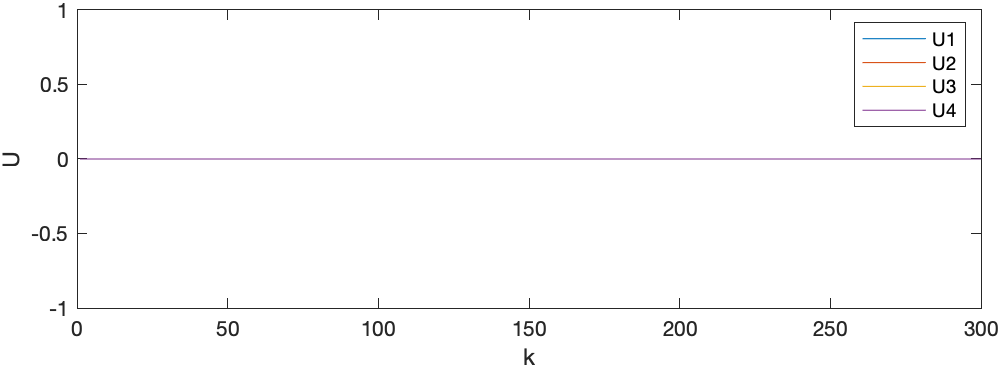
\includegraphics[scale=0.7]{png/projekt/zad1_u.png}
	\caption{Wej�cia w punkcie pracy}
	\label{zad1_u}
\end{figure}
 
 \begin{figure}[H]
 	\centering
 	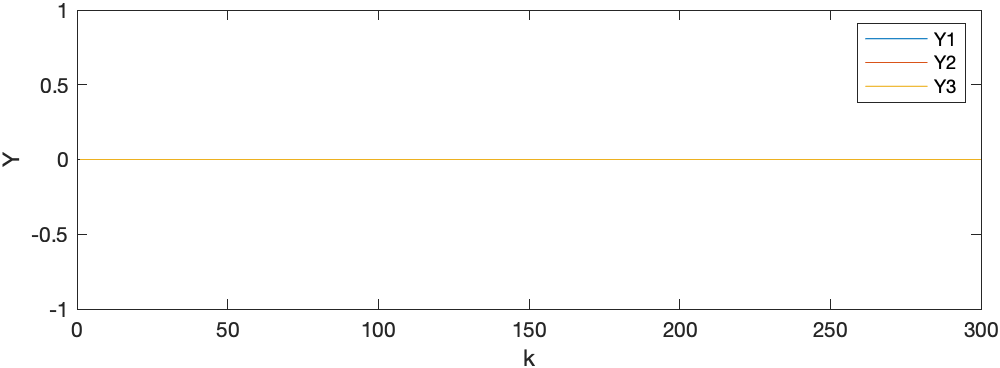
\includegraphics[scale=0.7]{png/projekt/zad1_y.png}
 	\caption{Wyj�cia w punkcie pracy}
 	\label{zad1_y}
 \end{figure}
\section{Wyznaczenie odpowiedzi skokowych procesu}

\textcolor{red}{TODO OPISA�}

 \begin{figure}[H]
	\centering
	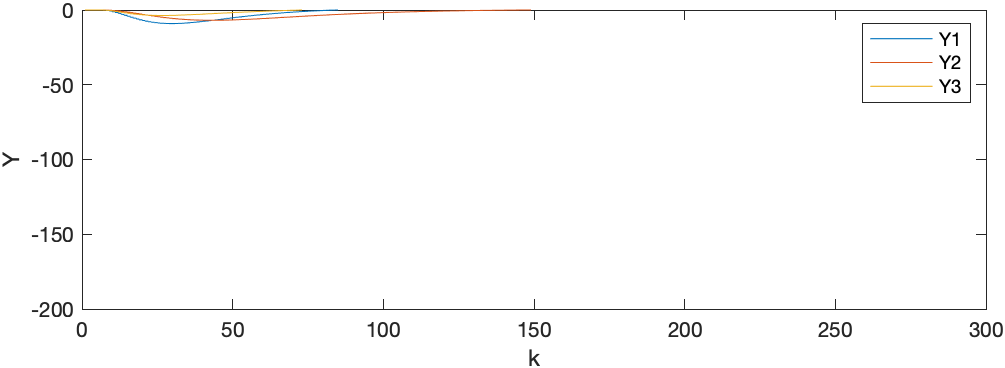
\includegraphics[scale=0.7]{png/projekt/zad2_u1.png}
	\caption{Odpowiedzi skokowe dla $U_1 = 1$}
	\label{zad2_u1}
\end{figure}

 \begin{figure}[H]
	\centering
	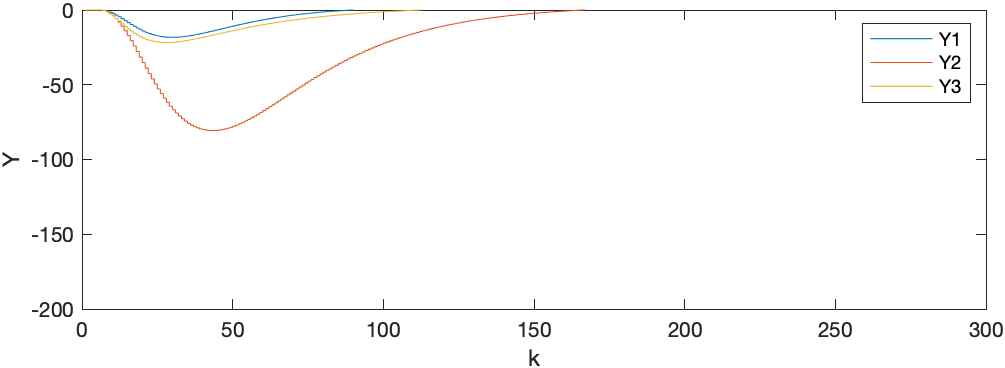
\includegraphics[scale=0.7]{png/projekt/zad2_u2.png}
	\caption{Odpowiedzi skokowe dla $U_2 = 1$}
	\label{zad2_u2}
\end{figure}

 \begin{figure}[H]
	\centering
	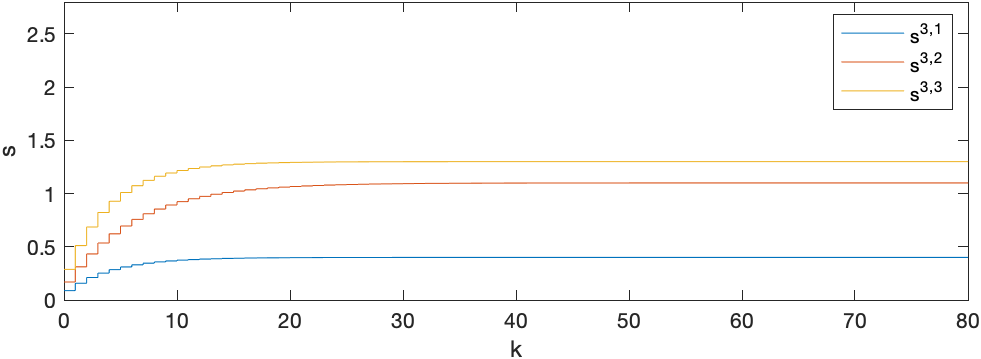
\includegraphics[scale=0.7]{png/projekt/zad2_u3.png}
	\caption{Odpowiedzi skokowe dla $U_3 = 1$}
	\label{zad2_u3}
\end{figure}

 \begin{figure}[H]
	\centering
	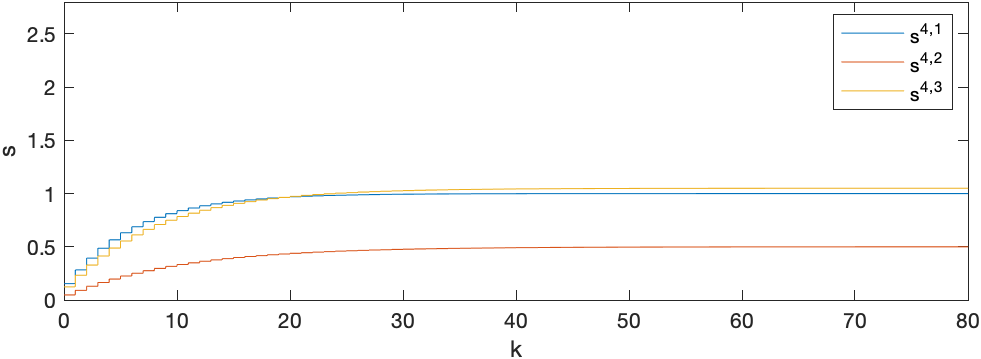
\includegraphics[scale=0.7]{png/projekt/zad2_u4.png}
	\caption{Odpowiedzi skokowe dla $U_4 = 1$}
	\label{zad2_u4}
\end{figure}

\section{Algorytm PID}



\section{Algorytm DMC w wersji analitycznej}

\section{Algorytm DMC w wersji klasycznej}




